\subsection{Scaling with divergence}\label{app:scaling-e}

\Cref{fig:scaling-e-zoom} shows the runtime scaling with divergence for various
heuristics. The heuristics using inexact matches ($r{=}2$) are slower for
low-divergence sequences due to spending relatively a lot of time on the
initialization of the heuristic, which requires finding all inexact matches.

The threshold for near-constant runtime is near $10\% = 1/k$ for exact matches
and near $20\% = 2/k$ for inexact matches. As the divergence approaches this
threshold, the runtime (and number of expanded states) starts to grow. This can
be explained as follows.

For each error that is not accounted for by a heuristic, \A needs to increase
its best estimate $f$ of the total cost by $1$. This means it needs to
\emph{backtrack} and expand more states with this higher $f$ value, including
states before the search tip. Pruning compensates for this by increasing $h$
before the tip. However, the more unaccounted errors occur, the more pruned
matches are needed. Once the total cost is equal to the potential, \emph{all}
pruned matches are needed to compensate. At that point, each edit that is not
accounted for effectively increases the band width by $2$.

\begin{figure}[H]
  \centering
  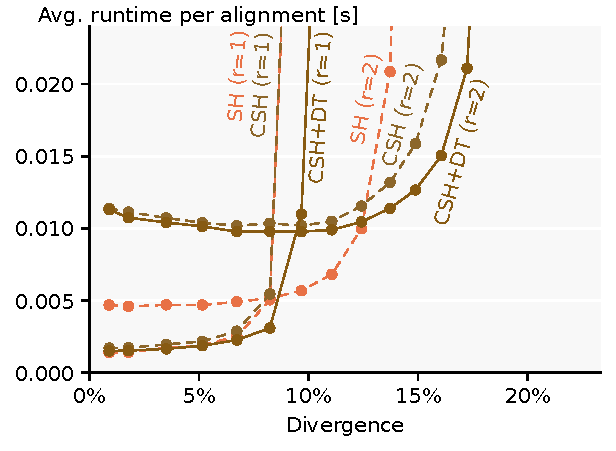
\includegraphics[scale=0.6]{plots/scaling_e_zoom.labels.pdf}
  \caption[Runtime scaling with divergence (zoomed)]{\textbf{Runtime scaling
    with divergence (zoomed)} (linear, synthetic, $n{=}10^4$, $10^6\bp$ total,
    $k{=}10$). The figure shows the same results as~\cref{fig:scaling-e}, but
    zoomed in to small runtimes where the scaling with $n$ degrades from linear
    to quadratic. $r{=}1$ and $r{=}2$ indicate exact and inexact matches,
    respectively.}
  \label{fig:scaling-e-zoom}
\end{figure}
